\documentclass[letterpaper]{article}
\usepackage[margin=1in]{geometry}
\usepackage[utf8]{inputenc}
\usepackage{textcomp}
\usepackage{amssymb}
\usepackage{natbib}
\usepackage{graphicx}
\usepackage{gensymb}
\usepackage{amsthm, amsmath, mathtools}
\usepackage[dvipsnames]{xcolor}
\usepackage{enumerate}
\usepackage{mdframed}
\usepackage[most]{tcolorbox}
\usepackage{csquotes}
% https://tex.stackexchange.com/questions/13506/how-to-continue-the-framed-text-box-on-multiple-pages

\tcbuselibrary{theorems}

\newcommand{\R}{\mathbb{R}}
\newcommand{\Z}{\mathbb{Z}}
\newcommand{\N}{\mathbb{N}}
\newcommand{\Q}{\mathbb{Q}}
\newcommand{\C}{\mathbb{C}}
\newcommand{\code}[1]{\texttt{#1}}
\newcommand{\mdiamond}{$\diamondsuit$}
\newcommand{\PowerSet}{\mathcal{P}}
\newcommand{\Mod}[1]{\ (\mathrm{mod}\ #1)}
\DeclareMathOperator{\lcm}{lcm}

%\newtheorem*{theorem}{Theorem}
%\newtheorem*{definition}{Definition}
%\newtheorem*{corollary}{Corollary}
%\newtheorem*{lemma}{Lemma}
\newtheorem*{proposition}{Proposition}


\newtcbtheorem[number within=section]{theorem}{Theorem}
{colback=green!5,colframe=green!35!black,fonttitle=\bfseries}{th}

\newtcbtheorem[number within=section]{definition}{Definition}
{colback=blue!5,colframe=blue!35!black,fonttitle=\bfseries}{def}

\newtcbtheorem[number within=section]{corollary}{Corollary}
{colback=yellow!5,colframe=yellow!35!black,fonttitle=\bfseries}{cor}

\newtcbtheorem[number within=section]{lemma}{Lemma}
{colback=red!5,colframe=red!35!black,fonttitle=\bfseries}{lem}

\newtcbtheorem[number within=section]{example}{Example}
{colback=white!5,colframe=white!35!black,fonttitle=\bfseries}{def}

\newtcbtheorem[number within=section]{note}{Important Note}{
        enhanced,
        sharp corners,
        attach boxed title to top left={
            xshift=-1mm,
            yshift=-5mm,
            yshifttext=-1mm
        },
        top=1.5em,
        colback=white,
        colframe=black,
        fonttitle=\bfseries,
        boxed title style={
            sharp corners,
            size=small,
            colback=red!75!black,
            colframe=red!75!black,
        } 
    }{impnote}
\usepackage[utf8]{inputenc}
\usepackage[english]{babel}
\usepackage{fancyhdr}
\usepackage[hidelinks]{hyperref}

\pagestyle{fancy}
\fancyhf{}
\rhead{CSE 131}
\chead{Monday, April 24, 2023}
\lhead{Lecture 10}
\rfoot{\thepage}

\setlength{\parindent}{0pt}

\begin{document}

\section{Calling Conventions}
In this section, we'll talk more about calling conventions. 

\subsection{Argument Conventions in x86\_64}
Consider the following code (assuming that only this part of the code has changed.)
\begin{verbatim}
    #[link(name = "our_code")]
    extern "C" {
    #[link_name = "\x01our_code_starts_here"]
        fn our_code_starts_here(input : i64, p1 : i64, p2 : i64, ..., p8 : i64) -> i64;
    }

    fn main() {
        let args: Vec<String> = env::args().collect();
        let input = parse_arg(&args);
        let i : i64 = unsafe { 
            our_code_starts_here(input, 9, 10, 11, 12, 13, 14, 15, 16) 
        };
        snek_print(i);
    }\end{verbatim}
Here, we added 8 parameters to the \code{our\_code\_starts\_here} function so we can see how the arguments are represented in memory. Using \code{rust-lldb}, we can debug this code and, more importantly, see the memory layout of our program.
\begin{center}
    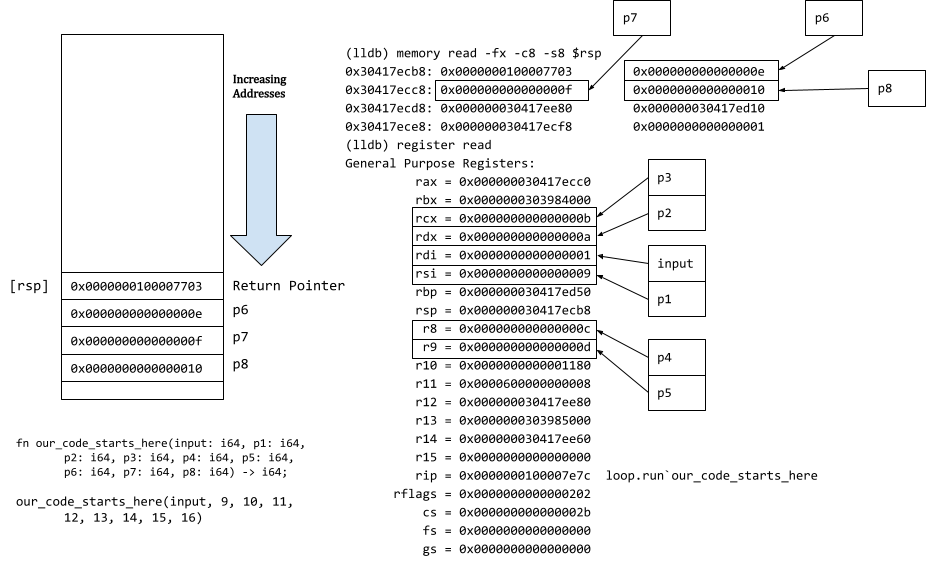
\includegraphics[scale=0.5]{../assets/mem_layout.png}
\end{center}
The main takeaways to get are, in x86\_64,
\begin{itemize}
    \item The first 6 arguments are \code{rdi}, \code{rsi}, \code{rdx}, \code{rcx}, \code{r8}, and \code{r9}.
    \item Any remaining arguments will go in order in increasing addresses \textbf{after} \code{[rsp]}, where \code{[rsp]} holds the return pointer.
\end{itemize}

\subsection{Functions \& Their Conventions for Us}
How do we add functions to our programming language? We need to restructure our programming langauge a bit. First, our program will have the following definition: 
\begin{verbatim}
    <prog> := <defn>* <expr>

    <defn> := (fun (<name> <name>) <expr>)
        | (fun (<name> <name> <name>) <expr>)

    <expr> := ... 
        | (<name> <expr>) 
        | (<name> <expr> <expr>)\end{verbatim}
In particular, 
\begin{itemize}
    \item \code{<prgm>} is what our \code{snek} file will look like. \code{<prgm>} is saying that it takes zero or more function definitions, and then the expression. So, past \code{snek} files had zero function definitions. Now, \code{snek} files can have more than zero function definitions.
    \item In our version of \code{<defn>}, 
    \begin{itemize}
        \item \code{(fun (<name> <name>) <expr>)} means that the function declaration has a \emph{name}, and then one argument after it, and then the following expression. 
        \item \code{(fun (<name> <name> <name>) <expr>)} means that the function declaration has a \emph{name}, and then \emph{two arguments} after the name, and then the following expression.
    \end{itemize}
    \item In \code{<expr>}, not only do we have the usual language features (e.g., numbers, identifiers, binary operations, etc.), but we also have support for calling the above functions. Specifically,
    \begin{itemize}
        \item \code{(<name> <expr>)} calls the function \code{<name>} with a single argument.
        \item \code{(<name> <expr> <expr>)} calls the function \code{<name>} with two arguments.
    \end{itemize}
\end{itemize}
Consider the following code. 
    \begin{verbatim}
    (fun (sumsquare x y)
        (+ (* x x) (* y y)))

    (sumsquare (* 2 input) (+ 30 (* 3 input)))\end{verbatim}
When \code{sumsquare} starts, we should expect the memory and stack to look something like:
\begin{center}
    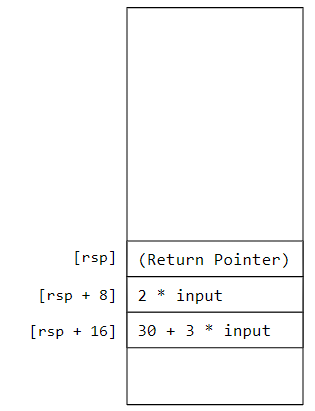
\includegraphics[scale=0.6]{../assets/function_mem_layout_dec.png}
\end{center}
In other words, the value of the first argument, $2 \times \code{input}$, when we called the function is in \code{[rsp + 8]}; likewise, the value of the second argument, $3 \times \code{input} + 30$, when we called the function is in \code{[rsp + 16]}. So, in general, how should we generate functions in our assembly code? 
\begin{itemize}
    \item For each function definition, we will generate a label. 
    \item Arguments will be located in the following places: 
    \begin{itemize}
        \item The value of the first argument is located in \code{[rsp + 8]}. 
        \item The value of the second argument is located in \code{[rsp + 16]}.
        \item In general, the value of the $i$th argument is located in \code{[rsp + 8(i + 1)]}.
    \end{itemize}
    This is controlled by the environment used for the body. 
\end{itemize}

Let's try to sketch out the assembly of the above code, where \code{sumsquare} is defined and where it is being called, and the corresponding memory model after running it. 

\begin{center}
    \begin{tabular}{p{3in}|p{3in}}
        \begin{verbatim}
; [rsp + 8] is x 
; [rsp + 16] is y
sumsquare:
    ; TODO 
    ret 

; basically, our main function 
our_code_starts_here:
    ; code for (* 2 input) -> rax 
    mov [rsp - 16], rax 
    ; code for (+ 30 (* 3 input))
    mov [rsp - 24], rax\end{verbatim}
        & \begin{center}
            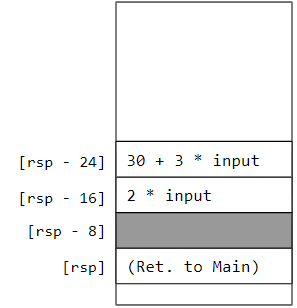
\includegraphics[scale=0.7]{../assets/sumsq_arg_order1.png}
        \end{center}
    \end{tabular}
\end{center}

\textbf{Notice} that the order of the arguments isn't correct, so we can't use the arguments as they appear right here. So, we need to do some more moving.

\begin{center}
    \begin{tabular}{p{3in}|p{3in}}
        \begin{verbatim}
; [rsp + 8] is x 
; [rsp + 16] is y
sumsquare:
    ; TODO 
    ret 

; basically, our main function 
our_code_starts_here:
    ; code for (* 2 input) -> rax 
    mov [rsp - 16], rax 
    ; code for (+ 30 (* 3 input))
    mov [rsp - 24], rax
    ; additional moves for args 
    sub rsp, 48 ; 8 * 6
                ; put at "top" of stack
    call sumsquare
    add rsp, 48\end{verbatim}
        & \begin{center}
            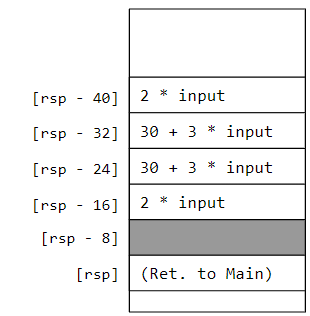
\includegraphics[scale=0.6]{../assets/sumsq_arg_order2.png}
        \end{center}
    \end{tabular}
\end{center}
We also may want to \textbf{save} any values that may be caller-saved (e.g., any registers like \code{rdi}). This should be done before doing any additional moves. Basically, we don't want to overwrite anything from a previous stack frame.

\subsection{Improvements and Approaches}
Some small ideas we could think about are: 
\begin{enumerate}
    \item The last argument can avoid copying. This is mainly so we can avoid doing some unnecessary minor work. 
    \item Evaluate arguments in reverse order (last to first). Then, they are in the right place on the stack. 
\end{enumerate}
Both of these run into issues with saving and restoring registers! So, a \textbf{big idea} is to \textbf{pre-allocate stack frames}\footnote{This is what Rust and C does.}. In other words, we move \code{rsp} at the \emph{start} of a function to accommodate \emph{all} local variables. Then, all references are \code{[rsp + \_\_\_]}. The interesting thing to think about is how much we need to move \code{rsp} to accommodate all local variables. Once we figure this out, then we can adjust \code{rsp} as needed. 

\bigskip 

Introducing, the \code{depth} function. This calculates the number of local variables (named or unnamed) are in this expression. This is basically just tracking stack indices. 
\begin{verbatim}
    fn depth(e: &Expr) -> i32 {
        match e {
            Plus(e1, e2) => {
                max(depth(e1), depth(e2) + 1)
            }
            Let(id, val, body) => {
                max(depth(val), depth(body) + 1)
            }
            ...
        }
    }\end{verbatim}
In a \code{Plus} expression, which has \code{e1} and \code{e2}, we're taking the maximum of 
\begin{itemize}
    \item \code{depth(e1)} (Because we don't increase the stack index when we go into \code{e1}), and 
    \item \code{depth(e2) + 1} (Remember that the plus expression makes space for one word, and then reserves that space while it's working on \code{e2}. This corresponds to how we did \code{si + 1} in our compiler.)
\end{itemize}
Analogously, we can say the same for the \code{Let} expression. 

\bigskip 

So, going back to compiling \code{sumsquare}, the first thing we can do is 
\begin{verbatim}
    sumsquare:
        sub rsp, depth(body * 8)
        . 
        . 
        .
        add rsp, depth(body * 8)
        ret\end{verbatim}
Note that all local variables use \code{[rsp + \_\_\_]} in this function. This means less calculations and moving \code{rsp} at each call.

\end{document}